\chapter{周期信号的频谱测试}%
\label{cha:周期信号的频谱测试}

\section{实验目的}%
\label{sec:实验目的\arabic{chapter}}

\begin{enumerate}
	\item 掌握周期信号频谱的测试方法;
	\item 了解典型信号频谱的特点,建立典型信号的波形与频谱之间的关系。
\end{enumerate}

\section{实验原理及方法}%
\label{sec:实验原理及方法\arabic{chapter}}

\begin{enumerate}
	\item 信号的频谱可分为幅度谱、相位谱和功率谱,分别是将信号的基波和各次谐波的振幅、相位和功率按频率的高低依次排列而成的图形。
	\item 连续时间信号的频谱具有离散性、谐波性、收敛性。

		例如正弦波、周期矩形脉冲、三角波的幅度谱分别如图\ref{fig:正弦波波形和幅度谱}、\ref{fig:周期矩形脉冲的波形和幅度谱}、\ref{fig:三角波的波形和幅度谱}所示:

		\begin{enumerate}
			\item 正弦波的幅度谱如图\ref{fig:正弦波波形和幅度谱}所示。

				\begin{figure}[htpb]
					\centering
					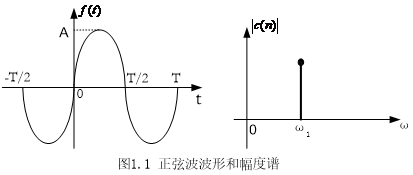
\includegraphics[width=0.8\linewidth]{1-2.png}
					\caption{正弦波波形和幅度谱}
					\label{fig:正弦波波形和幅度谱}
				\end{figure}

			\item 周期矩形脉冲的幅度谱如图\ref{fig:周期矩形脉冲的波形和幅度谱}所示。周期矩形脉冲的周期$ T $变化和$ \tau $变化时,幅度谱如图\ref{fig:周期矩形脉冲的波形和幅度谱的变化}所示。

				\begin{figure}[htpb]
					\centering
					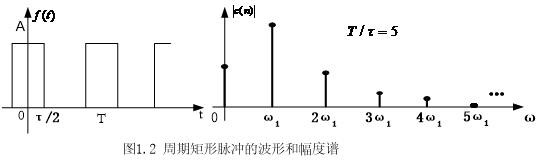
\includegraphics[width=0.8\linewidth]{1-2a.png}
					\caption{周期矩形脉冲的波形和幅度谱}
					\label{fig:周期矩形脉冲的波形和幅度谱}
				\end{figure}

				\begin{figure}[htpb]
					\centering
					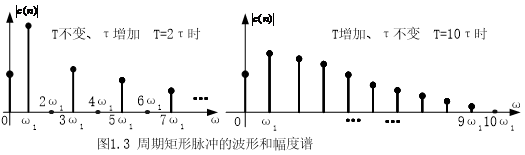
\includegraphics[width=0.8\linewidth]{1-2a2.png}
					\caption{周期矩形脉冲的波形和幅度谱的变化}
					\label{fig:周期矩形脉冲的波形和幅度谱的变化}
				\end{figure}

			\item 三角波的幅度谱如图1.4所示。

				\begin{figure}[htpb]
					\centering
					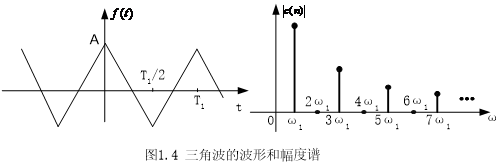
\includegraphics[width=0.8\linewidth]{1-2b.png}
					\caption{三角波的波形和幅度谱}
					\label{fig:三角波的波形和幅度谱}
				\end{figure}

				因此,频谱的测试方法可用频谱分析仪直接测量亦可用逐点测量法进行测量。本实验中使用逐点测量法测量幅度谱。所谓逐点测量法就是按频率由低到高将输入信号的各谐波分量一个一个地测量出来。测量中使用的仪器为选频电平表,选频电平表有两种型号,分别为HX-D21型和YX5014型,其使用方法见附录A。
		\end{enumerate}
\end{enumerate}

\section{实验前预习内容}%
\label{sec:实验前预习内容\arabic{chapter}}

\begin{Exercise}
	计算重复频率为\SI{500}{Hz}的方波、三角波的频谱,并画出频谱图\ref{fig:方波频谱图}、\ref{fig:三角波频谱图}。
\end{Exercise}

\begin{Answer}
	见图\subref{fig:方波频谱图}和\subref{fig:三角波频谱图}。
\end{Answer}

\begin{Exercise}
	计算重复频率为\SI{500}{Hz}、脉冲宽度分别为\SI{0.4}{ms}和\SI{1}{ms}的对称矩形脉冲的频谱,并画出频谱图\ref{fig:对称矩形脉冲频谱图1}、\ref{fig:对称矩形脉冲频谱图2};
\end{Exercise}

\begin{Answer}
	见图\subref{fig:对称矩形脉冲频谱图1}和\subref{fig:对称矩形脉冲频谱图2}。
\end{Answer}

\begin{Exercise}
	利用Matlab画出频率分别为\SI{10}{kHz}与\SI{12}{kHz}的两正弦信号叠加的时域波形图\ref{fig:两正弦波叠加频谱图}。
\end{Exercise}

\begin{Answer}
	见图\subref{fig:两正弦波叠加频谱图}。
\end{Answer}


\langCVfile[Matlab][code:fseries.m][Matlab]{fseries.m}{src/fseries.m}

\langCVfile[Matlab][code:fseriesPlot.m][Matlab]{fseriesPlot.m}{src/fseriesPlot.m}

\langCVfile[Matlab][code:code13.m][Matlab]{code13.m}{src/code13.m}

\begin{figure}[htpb]
	\centering
	\matlablightfile{MATLAB Command Window}{src/code13.txt}
	\caption{运行界面}
	\label{fig:运行界面code13.m}
\end{figure}

\begin{figure}[htpb]
	\centering
	\begin{subfigure}[htpb]{.45\linewidth}
		\centering
		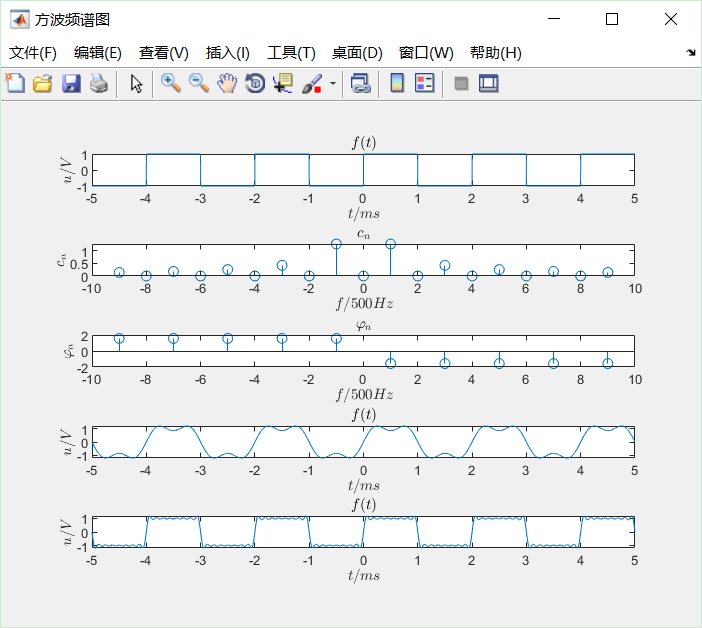
\includegraphics[width=\linewidth]{code131.png}
		\caption{方波频谱图}
		\label{fig:方波频谱图}
	\end{subfigure}
	\quad
	\begin{subfigure}[htpb]{.45\linewidth}
		\centering
		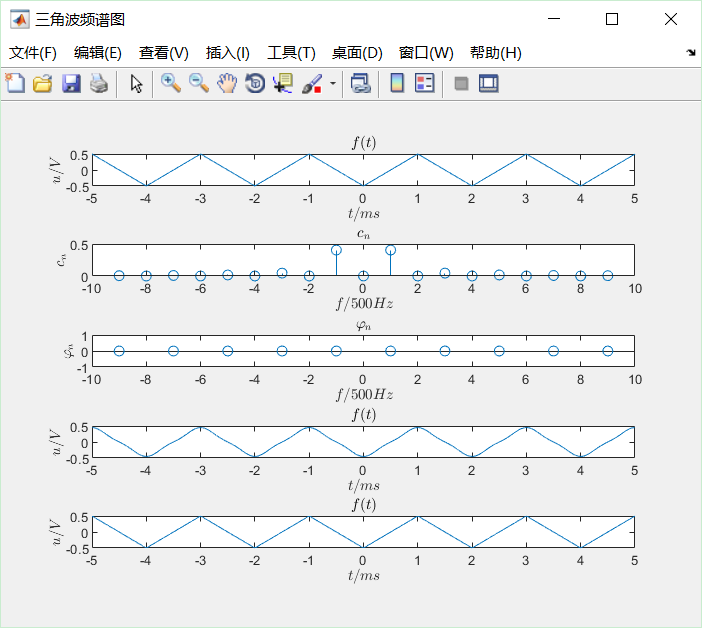
\includegraphics[width=\linewidth]{code132.png}
		\caption{三角波频谱图}
		\label{fig:三角波频谱图}
	\end{subfigure}

	\begin{subfigure}[htpb]{.45\linewidth}
		\centering
		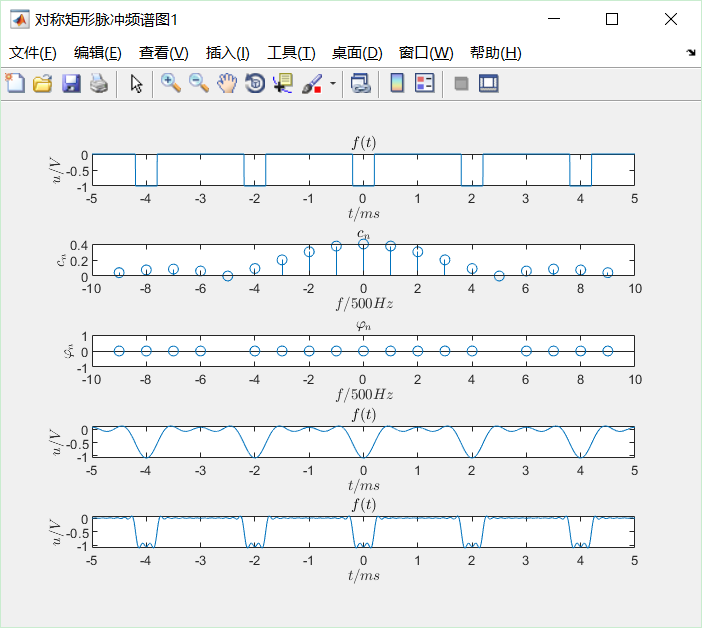
\includegraphics[width=\linewidth]{code133.png}
		\caption{对称矩形脉冲频谱图1}
		\label{fig:对称矩形脉冲频谱图1}
	\end{subfigure}
	\quad
	\begin{subfigure}[htpb]{.45\linewidth}
		\centering
		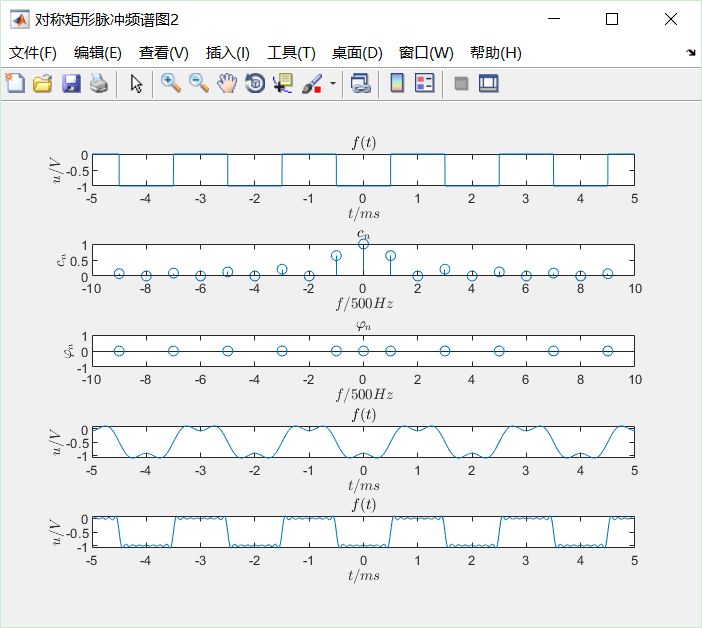
\includegraphics[width=\linewidth]{code134.png}
		\caption{对称矩形脉冲频谱图2}
		\label{fig:对称矩形脉冲频谱图2}
	\end{subfigure}
\end{figure}

\addtocounter{figure}{-1}
\begin{figure}[htpb]
	\centering
	\setcounter{sub}{\value{subfigure}}
	\begin{subfigure}[htpb]{.45\linewidth}
		\setcounter{subfigure}{\value{sub}}
		\centering
		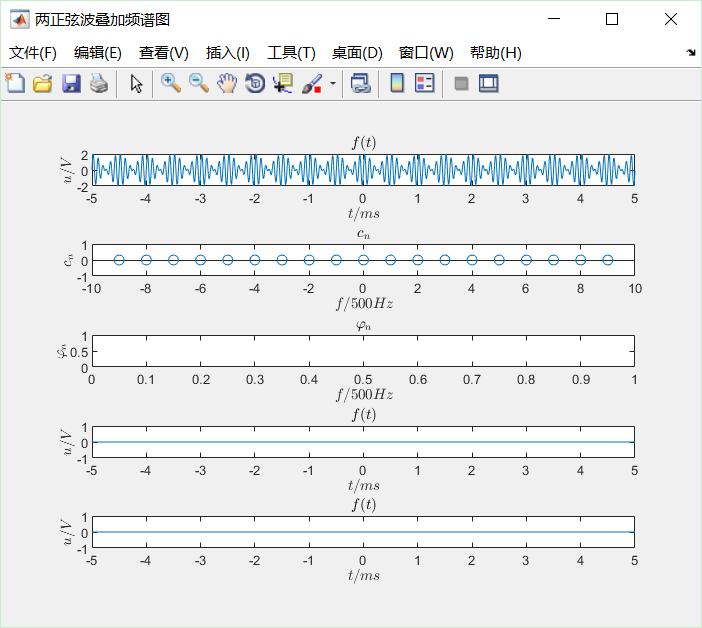
\includegraphics[width=\linewidth]{code135.png}
		\caption{两正弦波叠加频谱图}
		\label{fig:两正弦波叠加频谱图}
	\end{subfigure}
	\caption{频谱图}
	\label{fig:频谱图}
\end{figure}

\newpage

\section{实验原理图}%
\label{sec:实验原理图\arabic{chapter}}

\begin{figure}[htpb]
	\centering
	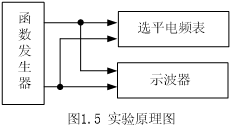
\includegraphics[width=0.6\linewidth]{1-4.png}
	\caption{实验原理图\arabic{chapter}}
	\label{fig:实验原理图\arabic{chapter}}
\end{figure}

\section{实验内容及步骤}%
\label{sec:实验内容及步骤\arabic{chapter}}

\subsection{测试对称方波的频谱}%
\label{sub:测试对称方波的频谱}

将信号源、示波器、选频电平表按图\ref{fig:实验原理图\arabic{chapter}}连接好;信号源输出CH1的输出波形调为方波(P),输出频率调为\SI{500}{Hz},输出信号幅度调为$ V_\text{\text{pp}}=\SI{10}{V} $,按附录A中介绍的选频电平表的使用方法将选频电平表的频率从\SI{200}{Hz}逐渐提高测出方波的前九次谐波分量。测量数据填入表\ref{tab:对称方波的前九次谐波幅度}。

\begin{figure}[htpb]
	\centering
	\begin{subfigure}[htpb]{.45\linewidth}
		\centering
		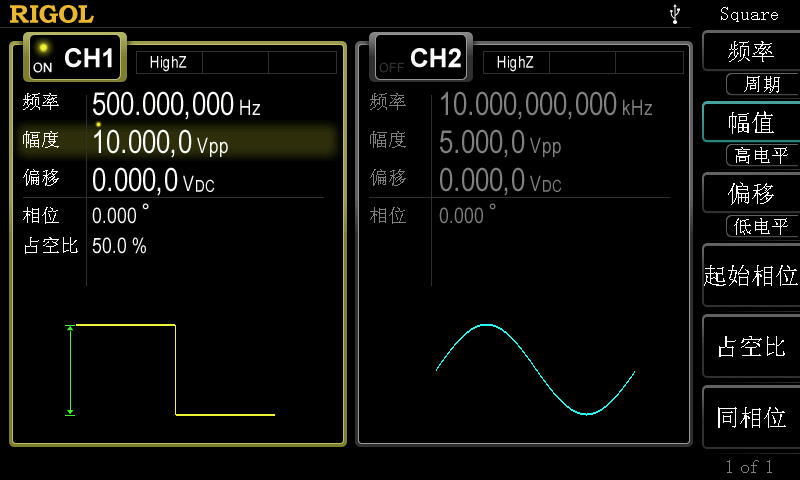
\includegraphics[width=\linewidth]{Rigol11.jpg}
		\caption{信号发生器输出对称方波}
		\label{fig:信号发生器输出对称方波}
	\end{subfigure}
	\quad
	\begin{subfigure}[htpb]{.45\linewidth}
		\centering
		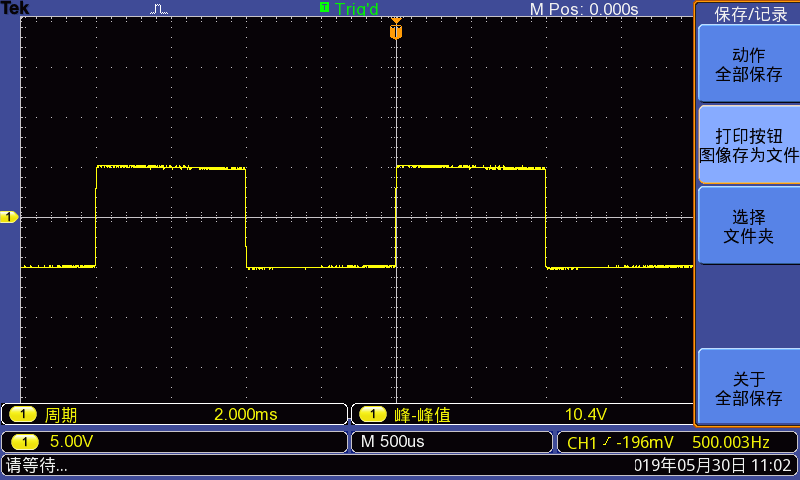
\includegraphics[width=\linewidth]{TEK11.png}
		\caption{示波器测量对称方波}
		\label{fig:示波器测量对称方波}
	\end{subfigure}
	\caption{对称方波}
	\label{fig:对称方波}
\end{figure}

\begin{table}[htpb]
	\centering
	\caption{对称方波的前九次谐波幅度}
	\label{tab:对称方波的前九次谐波幅度}
	\csvreader[
	head to column names,
	tabular=|c|c|c|c|c|c|c|c|c|c|,
	table head=\hline,
	late after line=\\\hline
	]{src/1-5-1.csv}{}{ \a&\b&\c&\d&\e&\f&\g&\h&\i&\j }
\end{table}

\subsection{测试三角波的频谱}%
\label{sub:测试三角波的频谱}

在实验步骤\ref{sub:测试对称方波的频谱}的基础上将信号源输出CH1的输出波形调为三角波(T),频率为\SI{1000}{Hz},幅度为$ V_\text{\text{pp}}=\SI{10}{V} $;用选频电平表测出前九次谐波分量。将测量数据填入表\ref{tab:三角波的前九次谐波幅度}。

\begin{figure}[htpb]
	\centering
	\begin{subfigure}[htpb]{.45\linewidth}
		\centering
		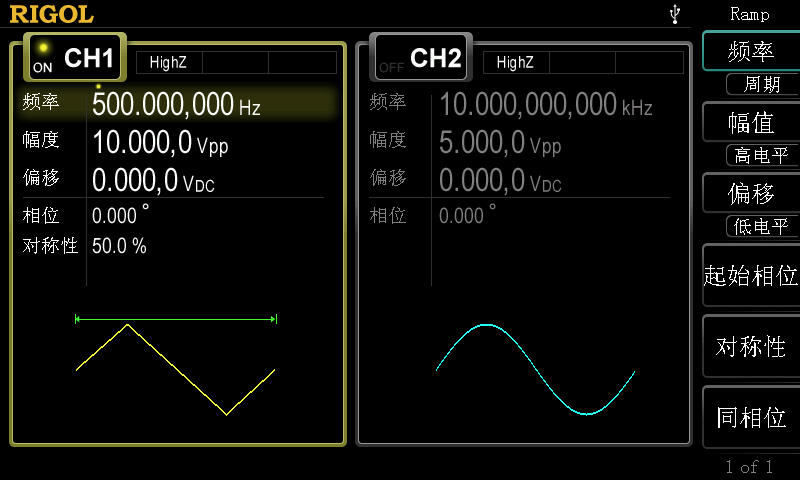
\includegraphics[width=\linewidth]{Rigol12.jpg}
		\caption{信号发生器输出三角波}
		\label{fig:信号发生器输出三角波}
	\end{subfigure}
	\quad
	\begin{subfigure}[htpb]{.45\linewidth}
		\centering
		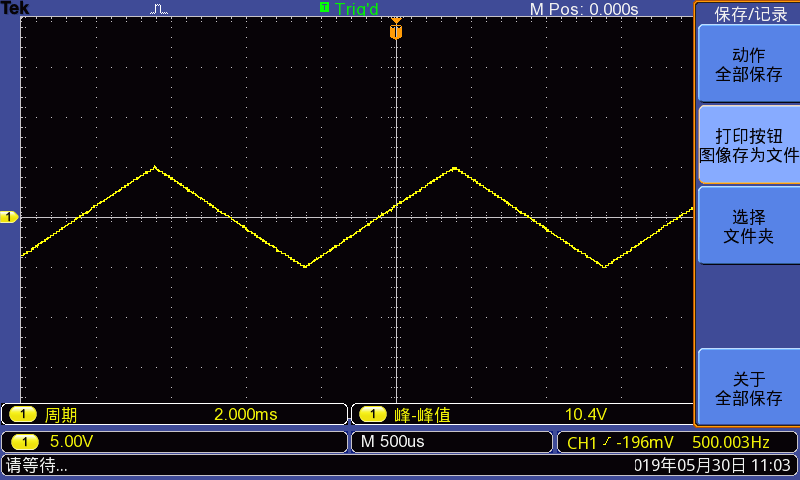
\includegraphics[width=\linewidth]{TEK12.png}
		\caption{示波器测量三角波}
		\label{fig:示波器测量三角波}
	\end{subfigure}
	\caption{三角波}
	\label{fig:三角波}
\end{figure}

\begin{table}[htpb]
	\centering
	\caption{三角波的前九次谐波幅度}
	\label{tab:三角波的前九次谐波幅度}
	\csvreader[
	head to column names,
	tabular=|c|c|c|c|c|c|c|c|c|c|,
	table head=\hline,
	late after line=\\\hline
	]{src/1-5-2.csv}{}{ \a&\b&\c&\d&\e&\f&\g&\h&\i&\j }
\end{table}

\subsection{测试周期矩形脉冲的频谱}%
\label{sub:测试周期矩形脉冲的频谱}

\begin{enumerate}
	\item 将信号源的输出线接“脉冲”输出端 ,信号周期(PP)调为\SI{2}{ms} ,脉宽(PW)调为\SI{0.4}{ms},用选频电平表测出信号的前九次谐波分量,填入表\ref{tab:周期矩形脉冲的前九次谐波幅度\arabic{enumi}}。

		\begin{figure}[htpb]
			\centering
			\begin{subfigure}[htpb]{.45\linewidth}
				\centering
				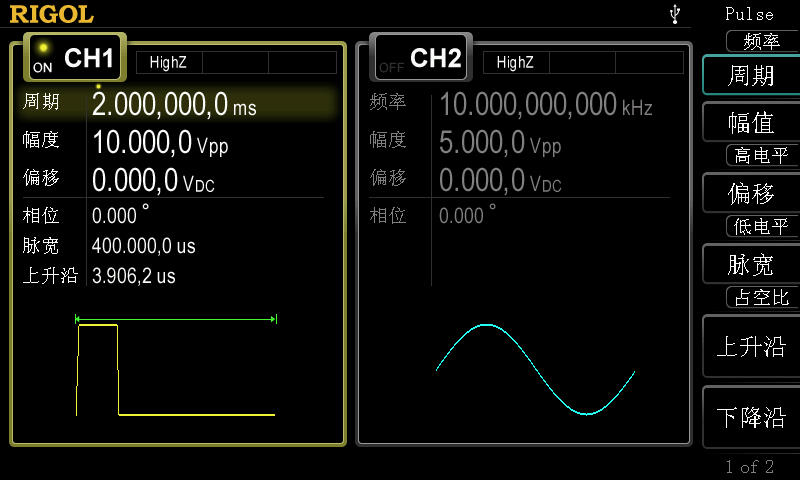
\includegraphics[width=\linewidth]{Rigol131.jpg}
				\caption{信号发生器输出周期矩形脉冲\arabic{enumi}}
				\label{fig:信号发生器输出周期矩形脉冲\arabic{enumi}}
			\end{subfigure}
			\quad
			\begin{subfigure}[htpb]{.45\linewidth}
				\centering
				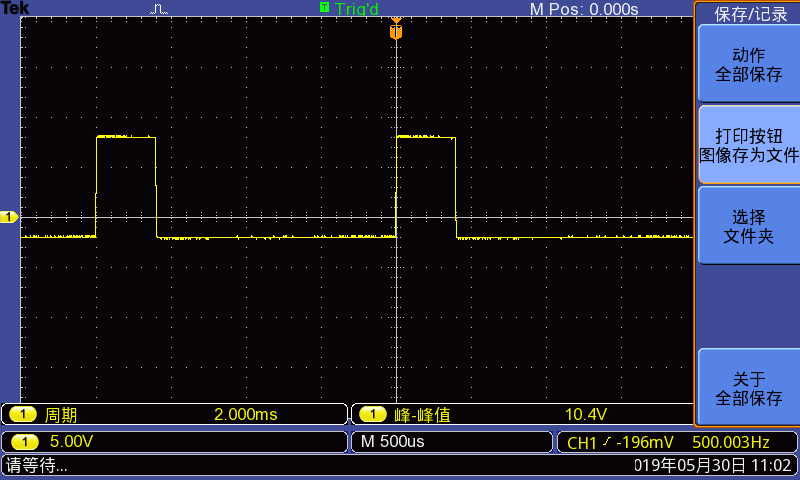
\includegraphics[width=\linewidth]{TEK131.png}
				\caption{示波器测量周期矩形脉冲\arabic{enumi}}
				\label{fig:示波器测量周期矩形脉冲\arabic{enumi}}
			\end{subfigure}
			\caption{周期矩形脉冲\arabic{enumi}}
			\label{fig:周期矩形脉冲\arabic{enumi}}
		\end{figure}

		\begin{table}[htpb]
			\centering
			\caption{周期矩形脉冲的前九次谐波幅度\arabic{enumi}}
			\label{tab:周期矩形脉冲的前九次谐波幅度\arabic{enumi}}
			\csvreader[
			head to column names,
			tabular=|c|c|c|c|c|c|c|c|c|c|,
			table head=\hline,
			late after line=\\\hline
			]{src/1-5-3.csv}{}{ \a&\b&\c&\d&\e&\f&\g&\h&\i&\j }
		\end{table}

	\item 将信号的脉宽(PW)调为\SI{1}{ms},周期保持不变,测出其前九次谐波分量,填入表\ref{tab:周期矩形脉冲的前九次谐波幅度\arabic{enumi}},并与内容\ref{sub:测试对称方波的频谱}进行比较。

		\begin{figure}[htpb]
			\centering
			\begin{subfigure}[htpb]{.45\linewidth}
				\centering
				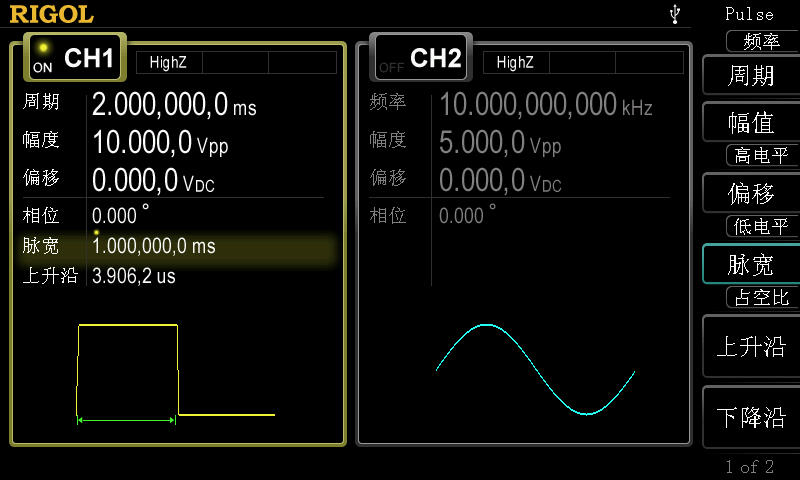
\includegraphics[width=\linewidth]{Rigol132.jpg}
				\caption{信号发生器输出周期矩形脉冲\arabic{enumi}}
				\label{fig:信号发生器输出周期矩形脉冲\arabic{enumi}}
			\end{subfigure}
			\quad
			\begin{subfigure}[htpb]{.45\linewidth}
				\centering
				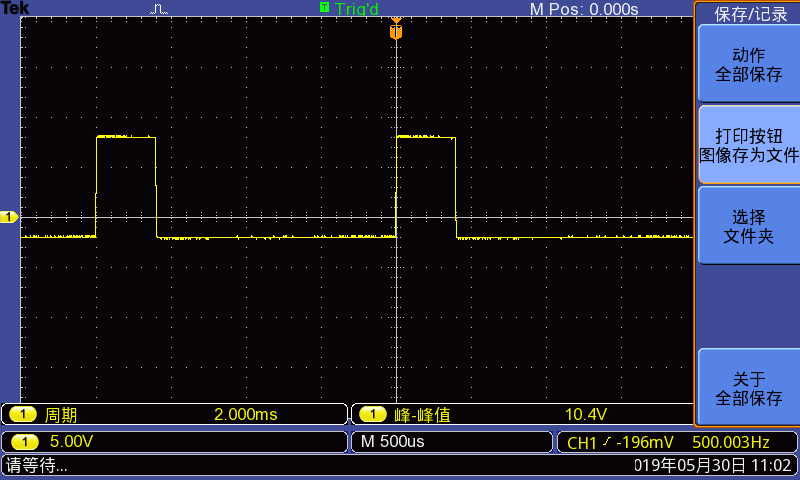
\includegraphics[width=\linewidth]{TEK131.png}
				\caption{示波器测量周期矩形脉冲\arabic{enumi}}
				\label{fig:示波器测量周期矩形脉冲\arabic{enumi}}
			\end{subfigure}
			\caption{周期矩形脉冲\arabic{enumi}}
			\label{fig:周期矩形脉冲\arabic{enumi}}
		\end{figure}

		\begin{table}[htpb]
			\centering
			\caption{周期矩形脉冲的前九次谐波幅度\arabic{enumi}}
			\label{tab:周期矩形脉冲的前九次谐波幅度\arabic{enumi}}
			\csvreader[
			head to column names,
			tabular=|c|c|c|c|c|c|c|c|c|c|,
			table head=\hline,
			late after line=\\\hline
			]{src/1-5-3a.csv}{}{ \a&\b&\c&\d&\e&\f&\g&\h&\i&\j }
		\end{table}
\end{enumerate}

\subsection{观测两正弦信号叠加后的波形及频谱}%
\label{sub:观测两正弦信号叠加后的波形及频谱}

将信号源按图\ref{fig:正弦信号叠加的原理图}所示连接好,并将输出波形均调为正弦波(S);

\begin{figure}[htpb]
	\centering
	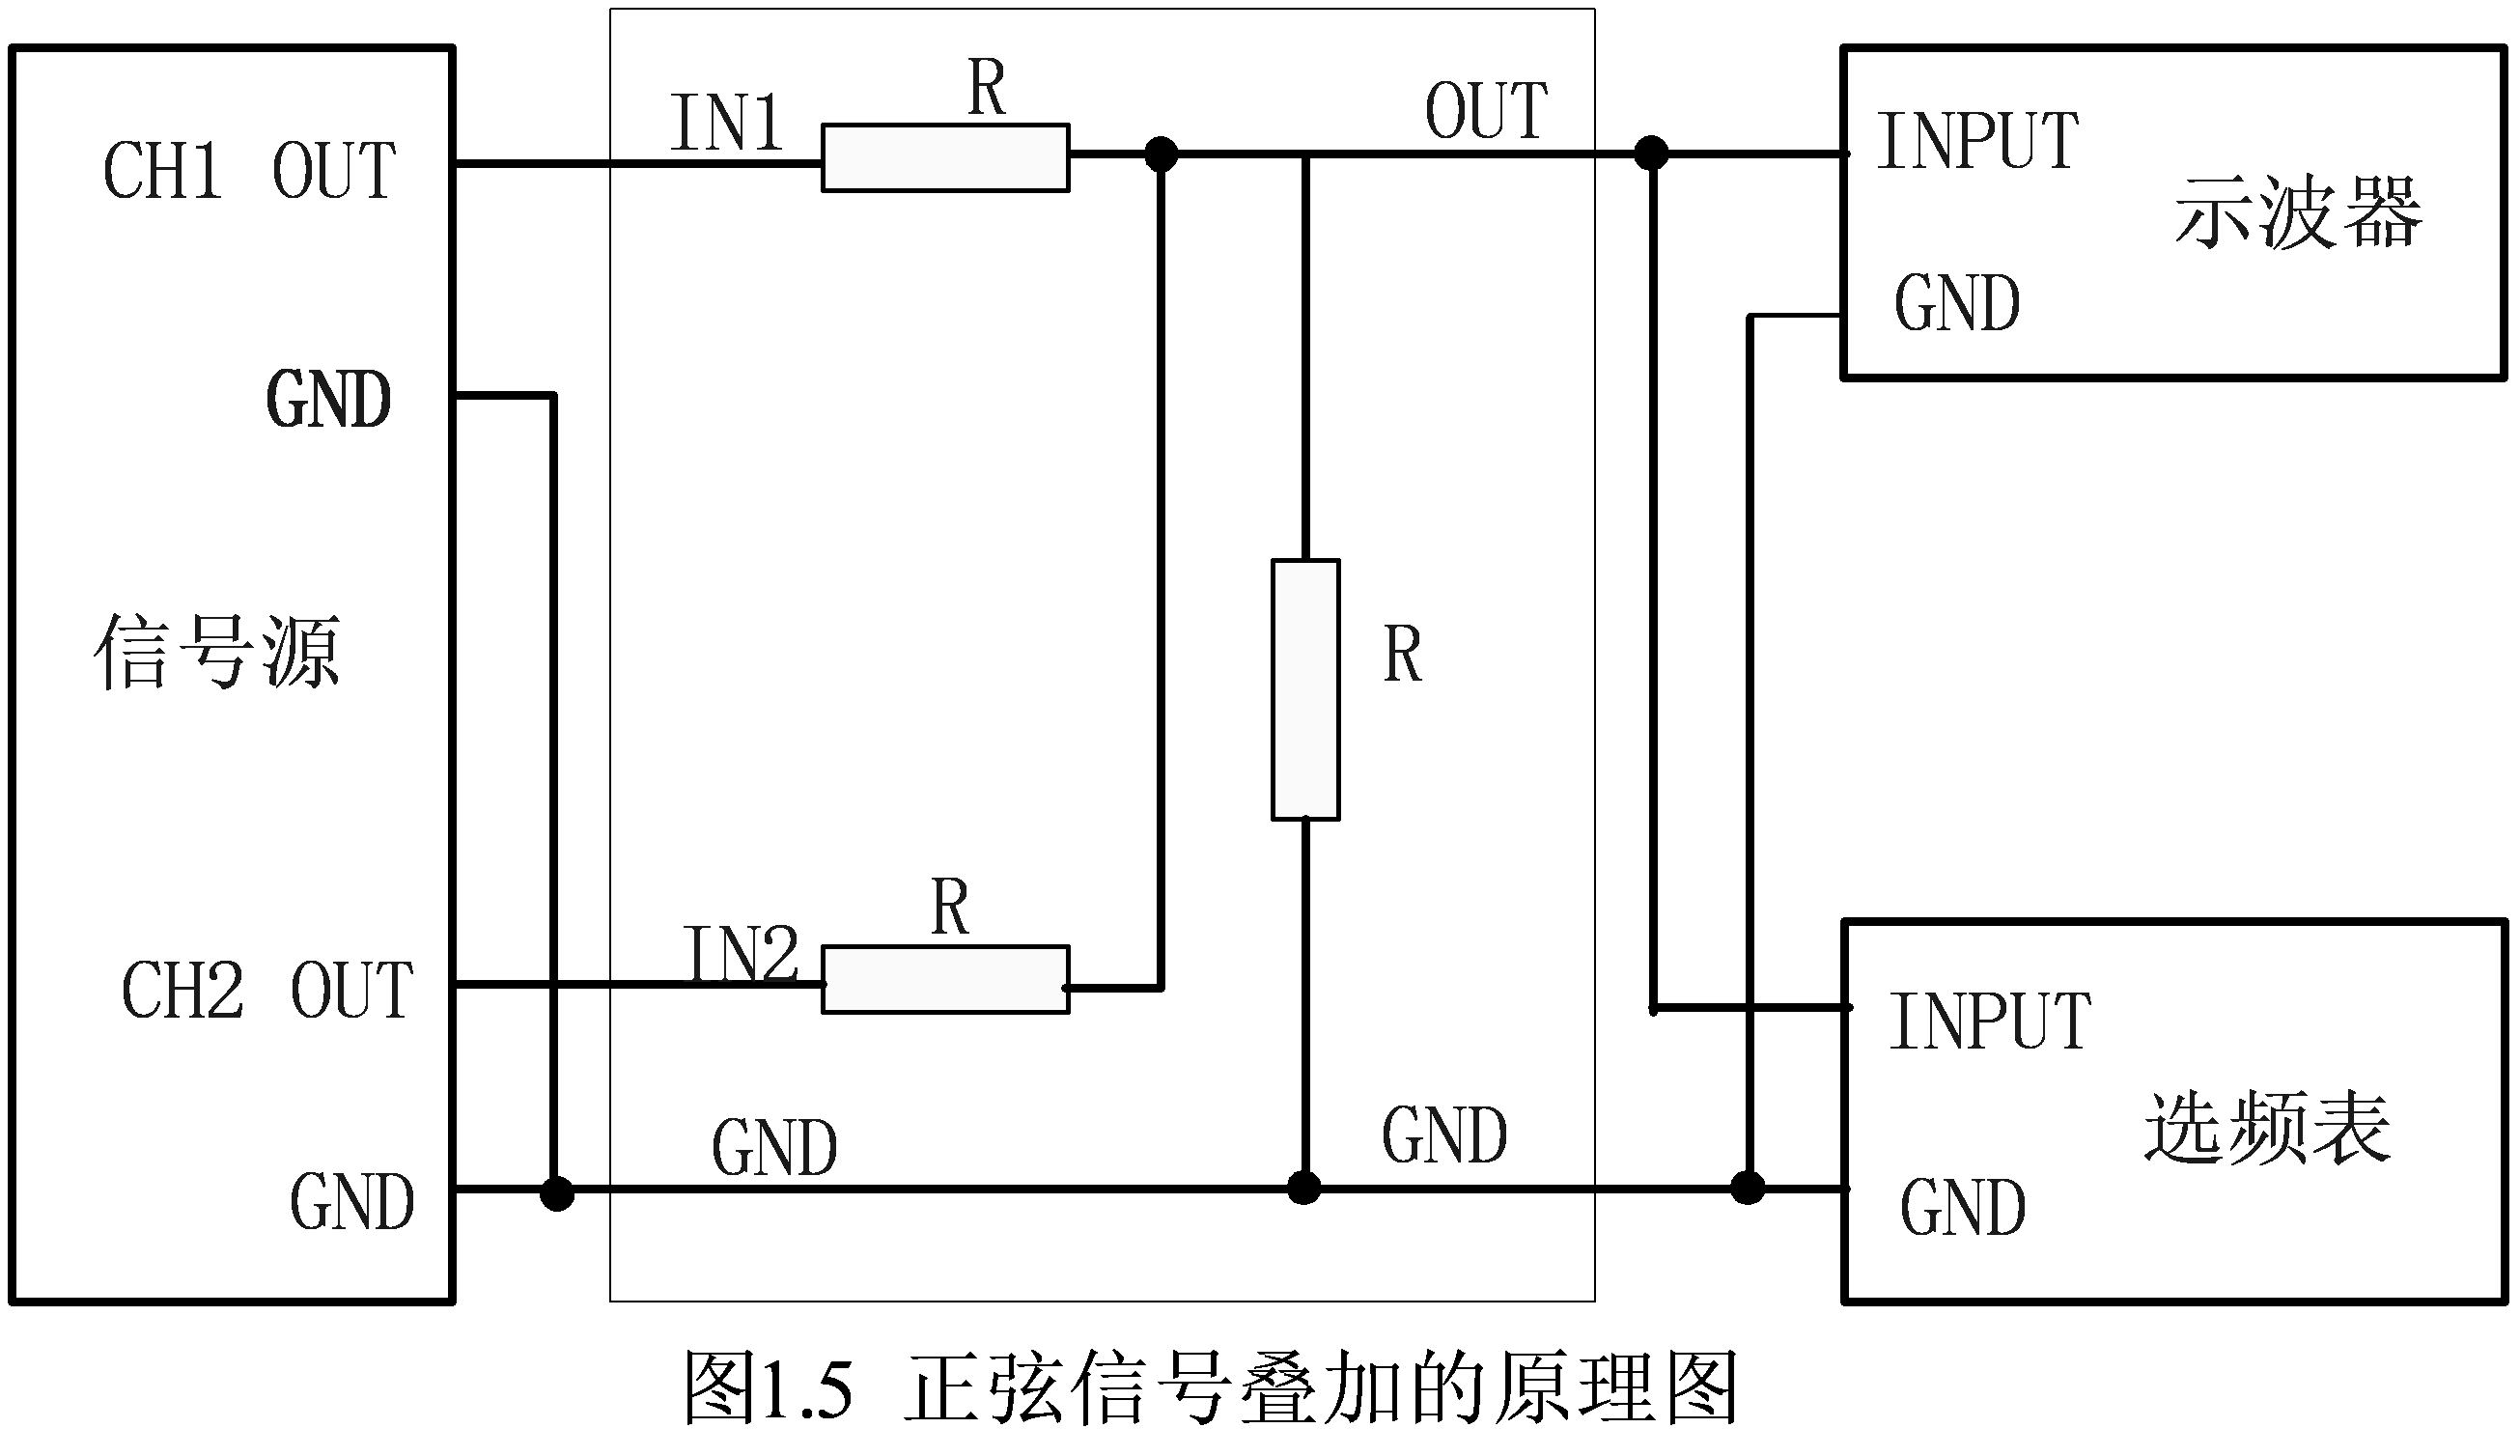
\includegraphics[width=0.6\linewidth]{1-5-4.png}
	\caption{正弦信号叠加的原理图}
	\label{fig:正弦信号叠加的原理图}
\end{figure}

\begin{enumerate}
	\item 再将信号源两路(CH1,CH2)的频率差距加大,即分别调为\SI{500}{Hz}和\SI{10}{kHz},幅度仍为$ V_{\text{pp}}=\SI{5}{V} $,观测示波器上的输出波形并记录,然后测出其频谱表\ref{tab:正弦信号叠加的频谱\arabic{enumi}},记录测量数据。

		\begin{table}[htpb]
			\centering
			\caption{正弦信号叠加的频谱\arabic{enumi}}
			\label{tab:正弦信号叠加的频谱\arabic{enumi}}
			\csvreader[
			head to column names,
			tabular=|c|c|c|,
			table head=\hline,
			late after line=\\\hline
			]{src/1-5-4.csv}{}{ \a&\b&\c }
		\end{table}

		\begin{figure}[htpb]
			\centering
			\begin{subfigure}[htpb]{.45\linewidth}
				\centering
				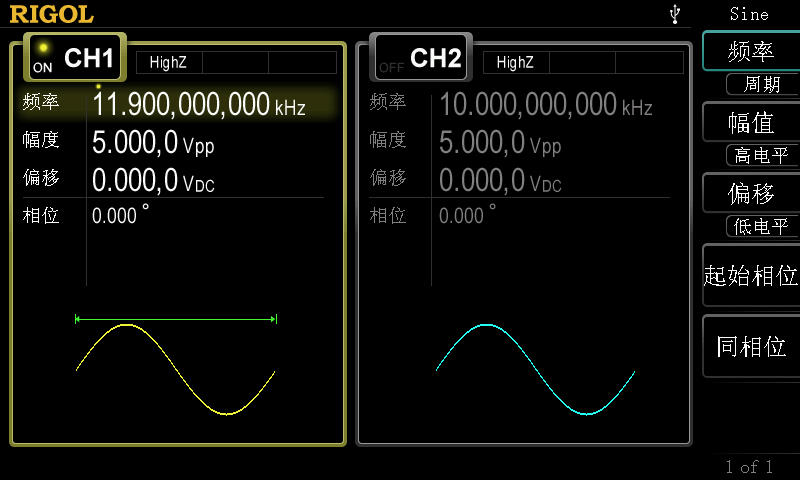
\includegraphics[width=\linewidth]{Rigol142.jpg}
				\caption{函数发生器输出两正弦信号叠加后的波形\arabic{enumi}}
				\label{fig:函数发生器输出两正弦信号叠加后的波形\arabic{enumi}}
			\end{subfigure}
			\quad
			\begin{subfigure}[htpb]{.45\linewidth}
				\centering
				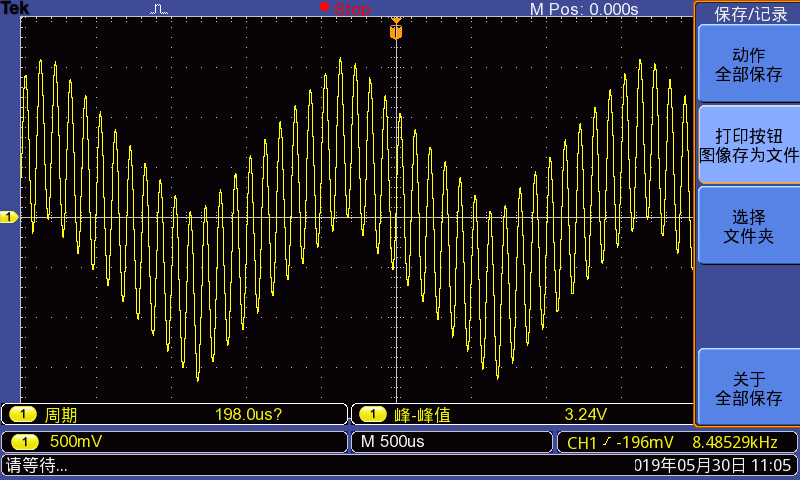
\includegraphics[width=\linewidth]{TEK141.png}
				\caption{示波器测量两正弦信号叠加后的波形\arabic{enumi}}
				\label{fig:示波器测量两正弦信号叠加后的波形\arabic{enumi}}
			\end{subfigure}
			\caption{两正弦信号叠加后的波形\arabic{enumi}}
			\label{fig:两正弦信号叠加后的波形\arabic{enumi}}
		\end{figure}

	\item 将信号源两路输出(CH1,CH2)的频率分别调为\SI{10}{kHz}和\SI{11.9}{kHz},信号幅度均调为$ V_\text{pp}=\SI{5}{V} $,观测示波器上的输出波形并定性记录,然后测出其频谱表\ref{tab:正弦信号叠加的频谱\arabic{enumi}},记录测量数据。

		\begin{figure}[htpb]
			\centering
			\begin{subfigure}[htpb]{.45\linewidth}
				\centering
				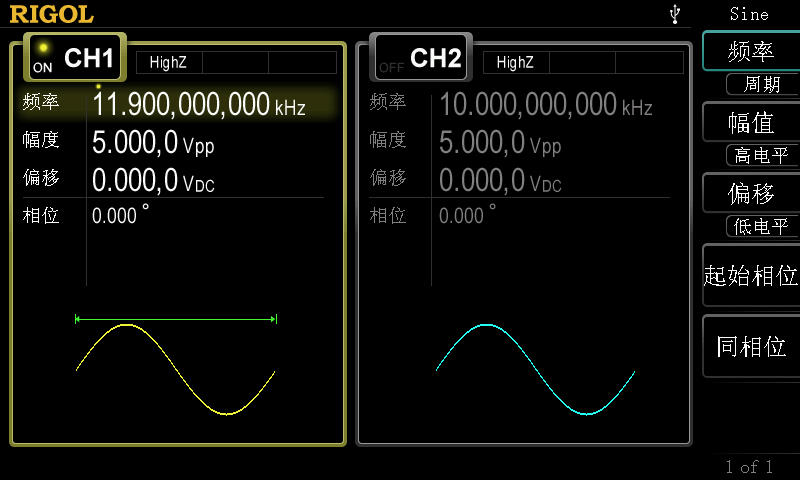
\includegraphics[width=\linewidth]{Rigol142.jpg}
				\caption{函数发生器输出两正弦信号叠加后的波形\arabic{enumi}}
				\label{fig:函数发生器输出两正弦信号叠加后的波形\arabic{enumi}}
			\end{subfigure}
			\quad
			\begin{subfigure}[htpb]{.45\linewidth}
				\centering
				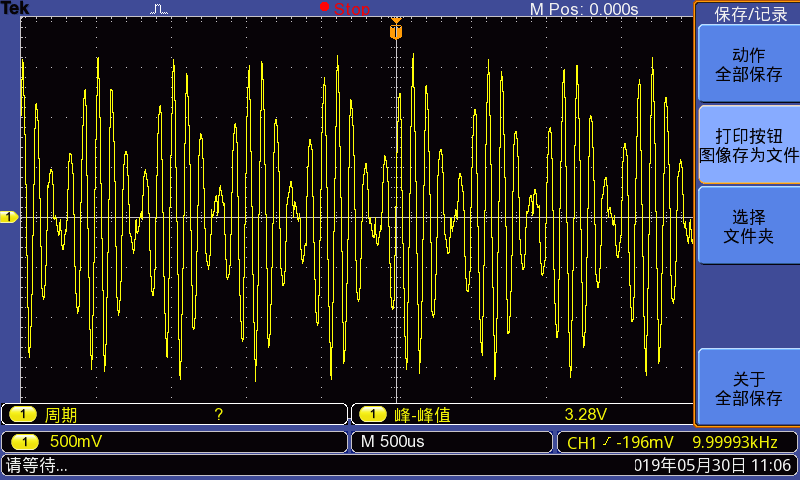
\includegraphics[width=\linewidth]{TEK142.png}
				\caption{示波器测量两正弦信号叠加后的波形\arabic{enumi}}
				\label{fig:示波器测量两正弦信号叠加后的波形\arabic{enumi}}
			\end{subfigure}
			\caption{两正弦信号叠加后的波形\arabic{enumi}}
			\label{fig:两正弦信号叠加后的波形\arabic{enumi}}
		\end{figure}

		\begin{table}[htpb]
			\centering
			\caption{正弦信号叠加的频谱\arabic{enumi}}
			\label{tab:正弦信号叠加的频谱\arabic{enumi}}
			\csvreader[
			head to column names,
			tabular=|c|c|c|,
			table head=\hline,
			late after line=\\\hline
			]{src/1-5-4a.csv}{}{ \a&\b&\c }
		\end{table}
\end{enumerate}

\section{实验仪器及设备}%
\label{sec:实验仪器及设备\arabic{chapter}}

双踪示波器一台,函数发生器一台,选频电平表一台,  实验板一块。

\section{实验报告要求}%
\label{sec:实验报告要求\arabic{chapter}}

\begin{Exercise}
	叙述实验内容及实验步骤。
\end{Exercise}

\begin{Answer}
	实验内容及步骤见第\ref{sec:实验内容及步骤\arabic{chapter}}节。
\end{Answer}

\begin{Exercise}
	整理实验数据,并根据实验数据画出频谱图。
\end{Exercise}

\begin{Answer}
	实验数据见表\ref{tab:对称方波的前九次谐波幅度}、\ref{tab:三角波的前九次谐波幅度}、\ref{tab:周期矩形脉冲的前九次谐波幅度1}、\ref{tab:周期矩形脉冲的前九次谐波幅度2}、\ref{tab:正弦信号叠加的频谱1}和\ref{tab:正弦信号叠加的频谱2}。频谱图见图\ref{fig:对称方波}、\ref{fig:三角波}、\ref{fig:周期矩形脉冲1}、\ref{fig:周期矩形脉冲2}、\ref{fig:两正弦信号叠加后的波形1}和\ref{fig:两正弦信号叠加后的波形2}。
\end{Answer}

\begin{Exercise}
	对实验内容\ref{sub:测试周期矩形脉冲的频谱}的实验数据进行分析并给出结论。
\end{Exercise}

\begin{Answer}
	当$ T $不变$ \tau $增加时幅度增加,间隔增加;当$ \tau $不变$ T $增加时幅度减小,间隔减小。
\end{Answer}

\begin{Exercise}
	画出实验中观测到的正弦信号叠加的波形,并将实验波形与仿真波形进行比较。
\end{Exercise}

\begin{Answer}
	观测波形见图\ref{fig:两正弦信号叠加后的波形1}和\ref{fig:两正弦信号叠加后的波形2},波形见图\ref{fig:两正弦波叠加频谱图},比较后发现仿真结果和实验比较吻合。
\end{Answer}

\begin{Exercise}
	说明不同频率正弦信号叠加后信号的特点。
\end{Exercise}

\begin{Answer}
	叠加后波形的形状与各信号的频率、初相、幅值有关,虽然不再是正弦信号,但一定是周期信号,且周期与最低频率分量的信号周期相同。
\end{Answer}

